\documentclass[11pt]{article}
\usepackage{graphicx}
\usepackage{caption}
\usepackage{float}
\usepackage{geometry}
\usepackage{booktabs}
\usepackage{amsmath}
\geometry{margin=1in}
\usepackage[colorlinks=true, linkcolor=blue, citecolor=blue, urlcolor=blue]{hyperref}

\title{Scientific Visualization Techniques: A Mini-Survey}

\author{
	Livan Miranda (6392173)\thanks{Team Leader} \and
	Rishav Sah (6499773)
}
\date{\today}
\vspace{3em}

\begin{document}
	
	\maketitle
	
	\begin{abstract}
		Scientific visualization transforms complex scientific data into visual formats that aid interpretation and analysis. This paper surveys the most common techniques used to visualize scalar and vector fields. We explore the strengths and limitations of each method and provide R-generated visualizations that demonstrate their use. Our findings highlight the importance of combining techniques for effective interpretation of multidimensional data.
	\end{abstract}
	
	\textbf{Keywords:} Scientific Visualization, Scalar Field Visualization, Vector Field Visualization, Slice Plane, Isosurface, Volume Rendering, Streamlines, R Graphics, Data Interpretation

	
	\section{Introduction}
	Scientific visualization is the graphical representation of data arising from scientific simulations and measurements. As datasets increase in size and complexity, visual techniques help scientists detect patterns, verify results, and communicate findings. Visualization is critical in fields such as physics, fluid dynamics, meteorology, and medicine.
	
	The data involved in visualization typically falls into two categories: \textbf{scalar fields}, which assign a single value (like temperature or pressure) to each point in space, and \textbf{vector fields}, which assign both magnitude and direction (like velocity or electromagnetic force).
	
	This mini-survey explores key methods for visualizing scalar and vector fields. We describe core techniques, illustrate them with graphs created using R, and assess their effectiveness. We also present a comparative table to evaluate strengths and limitations, and suggest best practices for combining methods.
	
	\section{Survey}
	
	\subsection{Scalar Field Visualization}
	Scalar fields represent data where each point in a domain is associated with a single numeric value. Effective visualization of such fields helps reveal trends, hot-spots, and boundaries as shown in Figure~\ref{fig:temperature_surface}.
	
	One of the most basic methods is the \textbf{slice plane}, which extracts a 2D cross-section of the 3D volume. Pseudocoloring is commonly used to encode scalar values on the slice using a gradient color map.
	
	The \textbf{isosurface} technique identifies all points in the domain with the same scalar value and connects them into a continuous surface. This is useful for threshold detection, such as identifying where pressure exceeds a critical value.
	
	\textbf{Volume rendering} displays the entire 3D domain as translucent layers, allowing scalar distributions to be viewed holistically. Proper use of opacity and lighting enables internal structures to emerge without slicing.
	
	\textbf{Scalar glyphs}, like colored disks or spheres, can be used to show value at sampled points. Though less common for dense datasets, they are helpful in sparse domains or on boundaries.
	
		\vspace{4em}
	
	\begin{figure}[H]
		\centering
		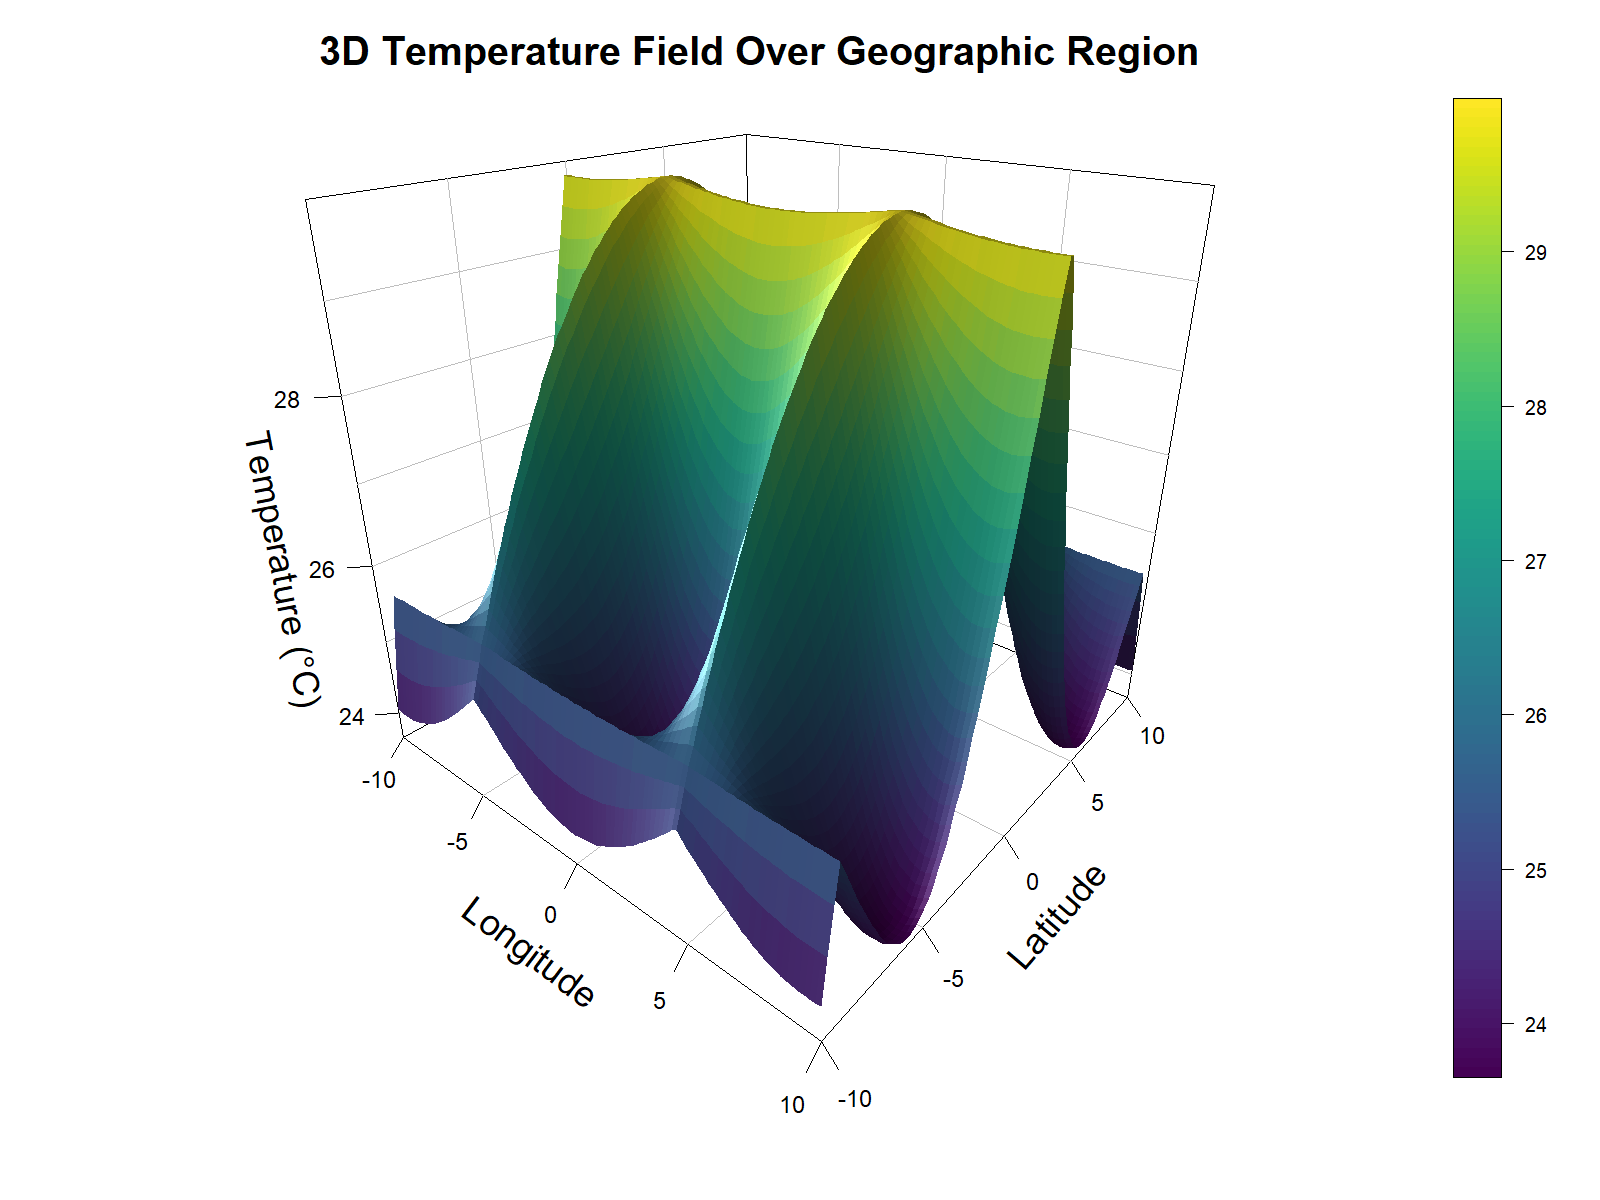
\includegraphics[width=0.85\textwidth]{temperature_surface_meteorology.png}
		\caption{Simulated 3D temperature field over a geographic region, modeling how temperature varies with latitude and terrain. This graph mimics real-world meteorological data used in climate and weather simulations.}
		\label{fig:temperature_surface}
	\end{figure}
	
	\vspace{1em}
	
	\noindent
	\textbf{Scenario:} \\
	This graph models temperature variation over a geographical area. The center of the domain represents a low-altitude, warmer zone, while surrounding regions simulate cooler temperatures due to elevation or latitude effects — much like real-world climate systems.
	
	\vspace{0.5em}
	\noindent
	\textbf{Simulated Meteorological Data:} \\
	The scalar values were generated using the following function:
	\[
	T(x, y) = 30 - \frac{y^2}{20} - \left|5 \cdot \cos\left(\frac{x}{3}\right) \cdot \sin\left(\frac{y}{3}\right)\right|
	\]
	Where:
	\begin{itemize}
		\item $x$ = longitude
		\item $y$ = latitude
	\end{itemize}
	
	This function creates a warmer central region (low elevation) and cooler outer regions (simulating higher elevation or polar effect). The oscillating sine-cosine term models terrain-like elevation-based temperature drops.
	
	\vspace{1em}
	\noindent
	\textbf{Relation to Scientific Visualization:} \\
	This plot represents a fundamental example of scalar field visualization, a core concept in scientific visualization. Scalar fields appear in many real-world domains, including:
	
	\begin{itemize}
	    \item Medical imaging (e.g., tissue density in CT/MRI scans)
	    \item Meteorology (e.g., temperature or pressure maps) 
	    \item Fluid dynamics (e.g., pressure distribution over a surface)
	    \item Geo-science (e.g., elevation or magnetic field intensity)
	\end{itemize}
	
	The use of both surface height and color to encode scalar values makes the data more interpretable. The 3D perspective adds spatial context and allows researchers to observe patterns, gradients, and critical regions in the data — which might be harder to identify in 2D views alone.
	
	\vspace{1em}
	\noindent
	\textbf{Why these techniques matters:} \\
	Scientists can understand abstract numerical data with scalar field visualization. These methods turn raw data into meaningful understanding, such as tumor density in medical scans, heat zones in engines, and pressure gradients in weather systems.
	

	\subsection{Vector Field Visualization}
	Vector fields assign both direction and magnitude to every point in space. These fields are typically used to model flow, force, or orientation, and require techniques that show movement and structure.
	
	\textbf{Vector glyphs} (e.g., arrows) are the simplest way to display direction and magnitude at specific points, but they become cluttered in dense regions.
	
	\textbf{Streamlines} offer a cleaner representation. These are lines that follow the tangent of the vector field and give a clear sense of flow direction.
	
	\textbf{Streaktubes} extend streamlines into tubes with 3D shading, making them easier to interpret spatially.
	
	\textbf{Ribbons} provide an additional twist dimension, representing how a small neighborhood of vectors twists in space. This is useful in identifying vorticity and turbulence.
	
	\vspace{1em}
	\noindent
	\textbf{Real-World Integration:} \\
	To demonstrate the application of vector field visualization with real-world data, we used wind speed data from the Open-Meteo API focused on the Miami region. The average wind value was used to simulate vertical lift, combined with a rotating horizontal field to mimic convection or vortex-like wind behavior. This resulted in 3D streamlines that visualize how directional wind flows propagate through space.
	
	Each streamline originates from a seed grid near the ground and is extended iteratively by calculating vector direction at each point. By using \texttt{rgl} in R, the field is visualized from three different angles (Figure~\ref{fig:wind_streamlines_1}–\ref{fig:wind_streamlines_3}) to better understand the vector dynamics.
	
	\vspace{1em}
	\textbf{Relation to Scientific Visualization:} \\
	This technique models and visualizes dynamic motion fields—commonly used in meteorology, fluid mechanics, and environmental modeling. It enhances interpretation of complex vector data by converting magnitude and direction into visual cues like curvature, density, and 3D orientation.
	
	\vspace{0.5em}
	
	\begin{figure}[H]
		\centering
		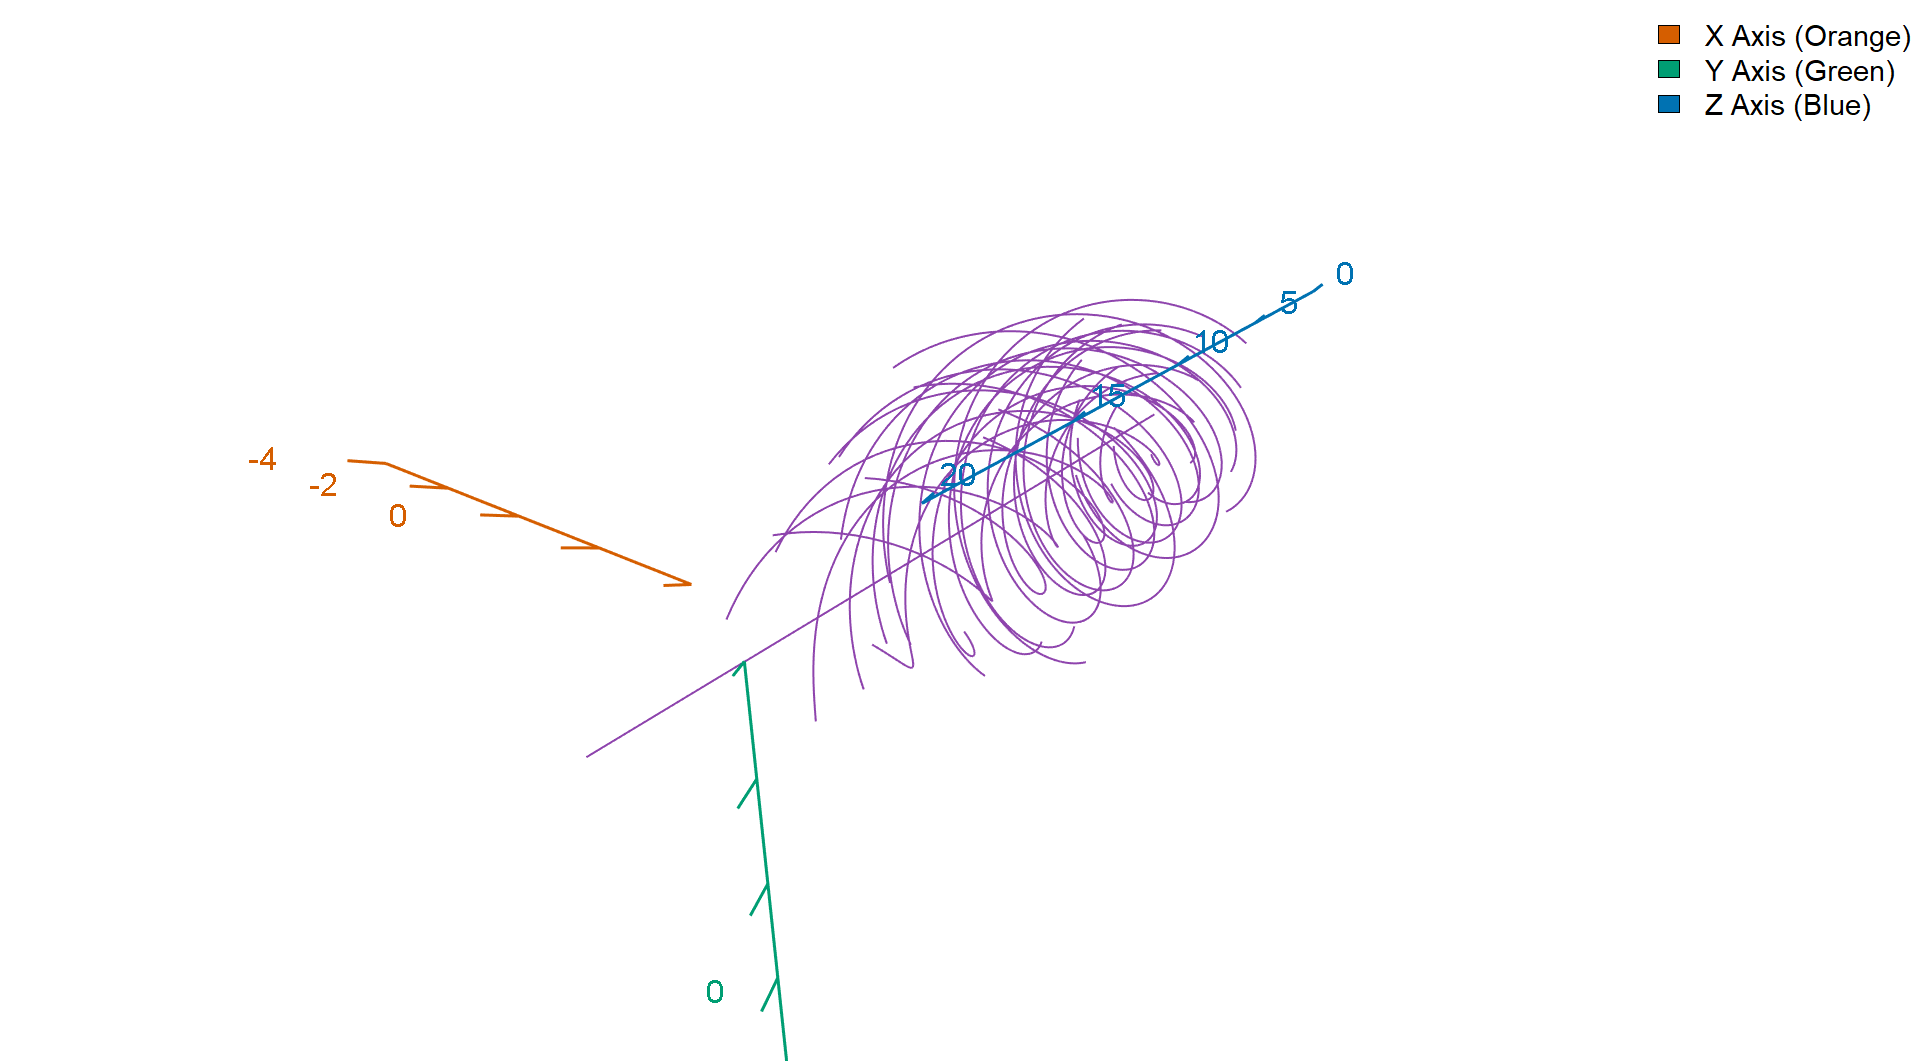
\includegraphics[width=0.85\textwidth]{vortex_view1.png}
		\caption{Real wind-based simulated 3D streamlines (View 1). Directional field based on windspeed data over Miami, showing upward and rotational flow structure.}
		\label{fig:wind_streamlines_1}
	\end{figure}
	
	\begin{figure}[H]
		\centering
		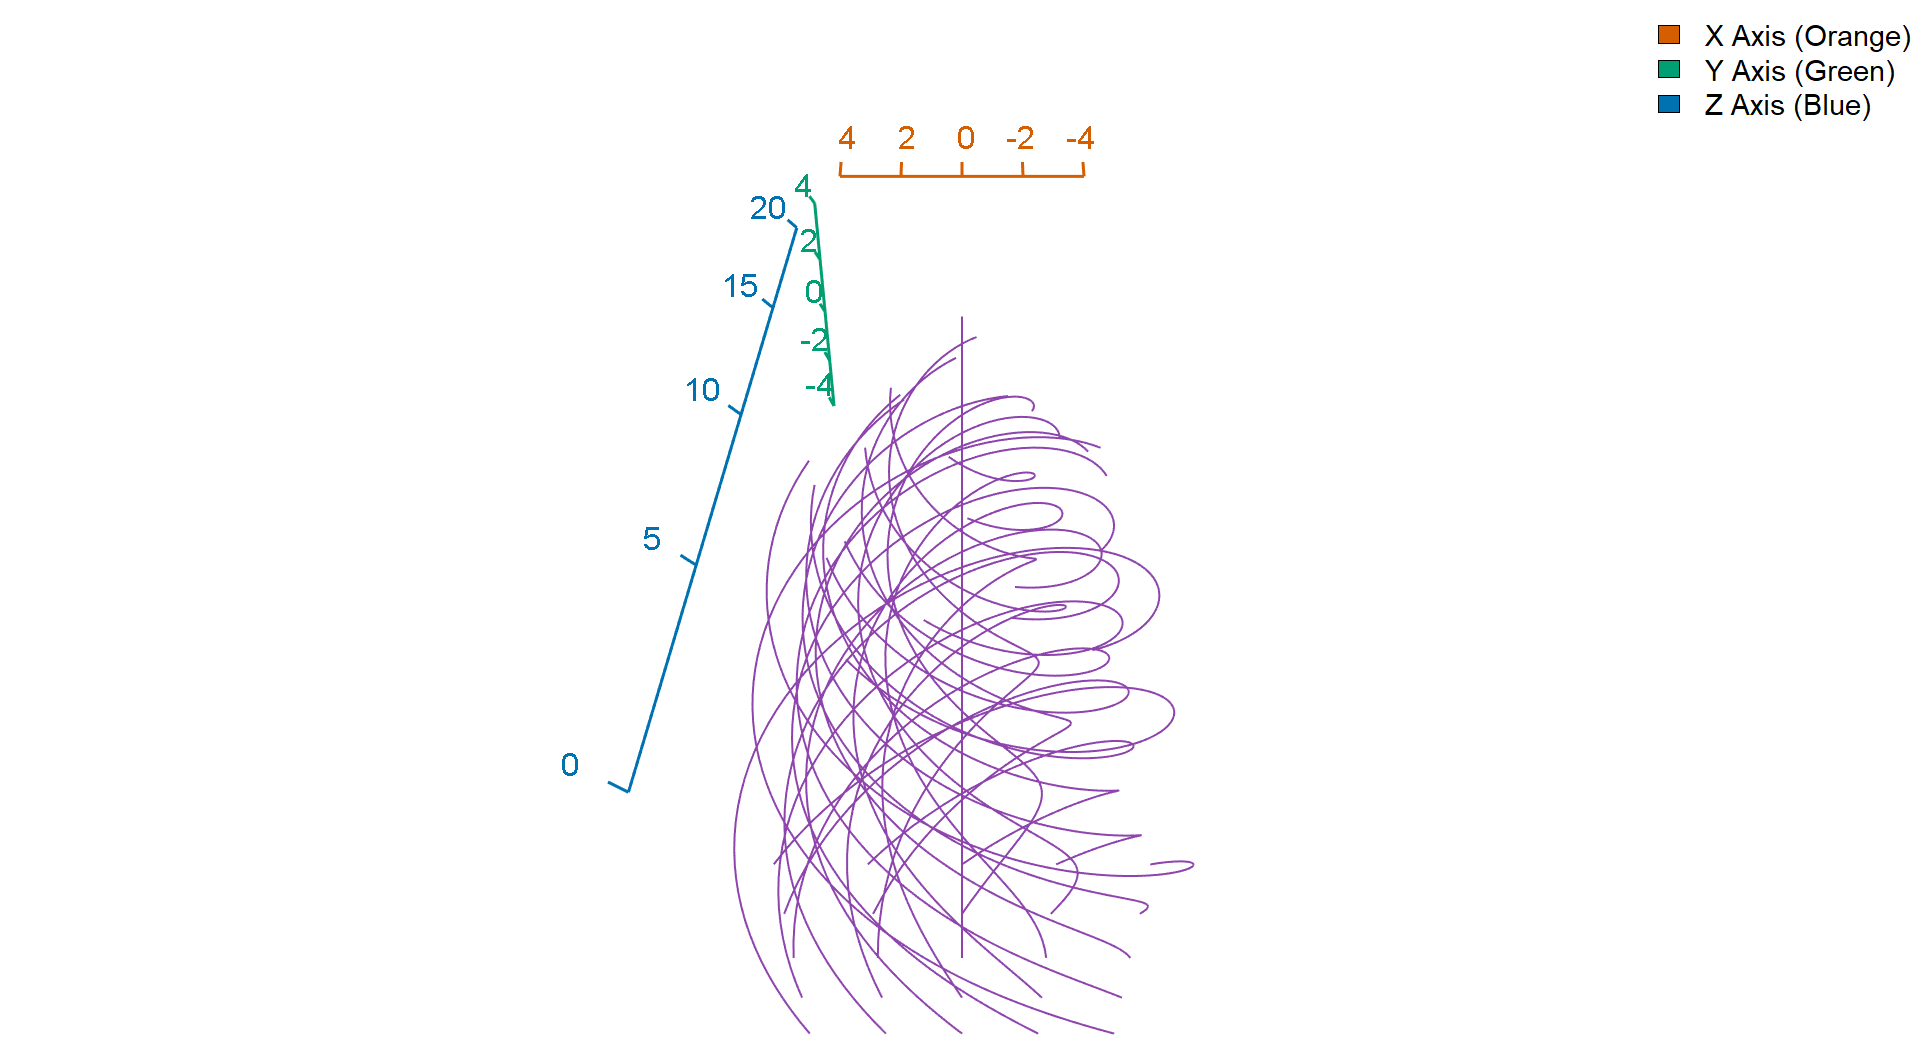
\includegraphics[width=0.85\textwidth]{vortex_view2.png}
		\caption{Alternate perspective (View 2) of the same wind-driven vector field. The structure illustrates flow curvature and 3D depth.}
		\label{fig:wind_streamlines_2}
	\end{figure}
	
	\begin{figure}[H]
		\centering
		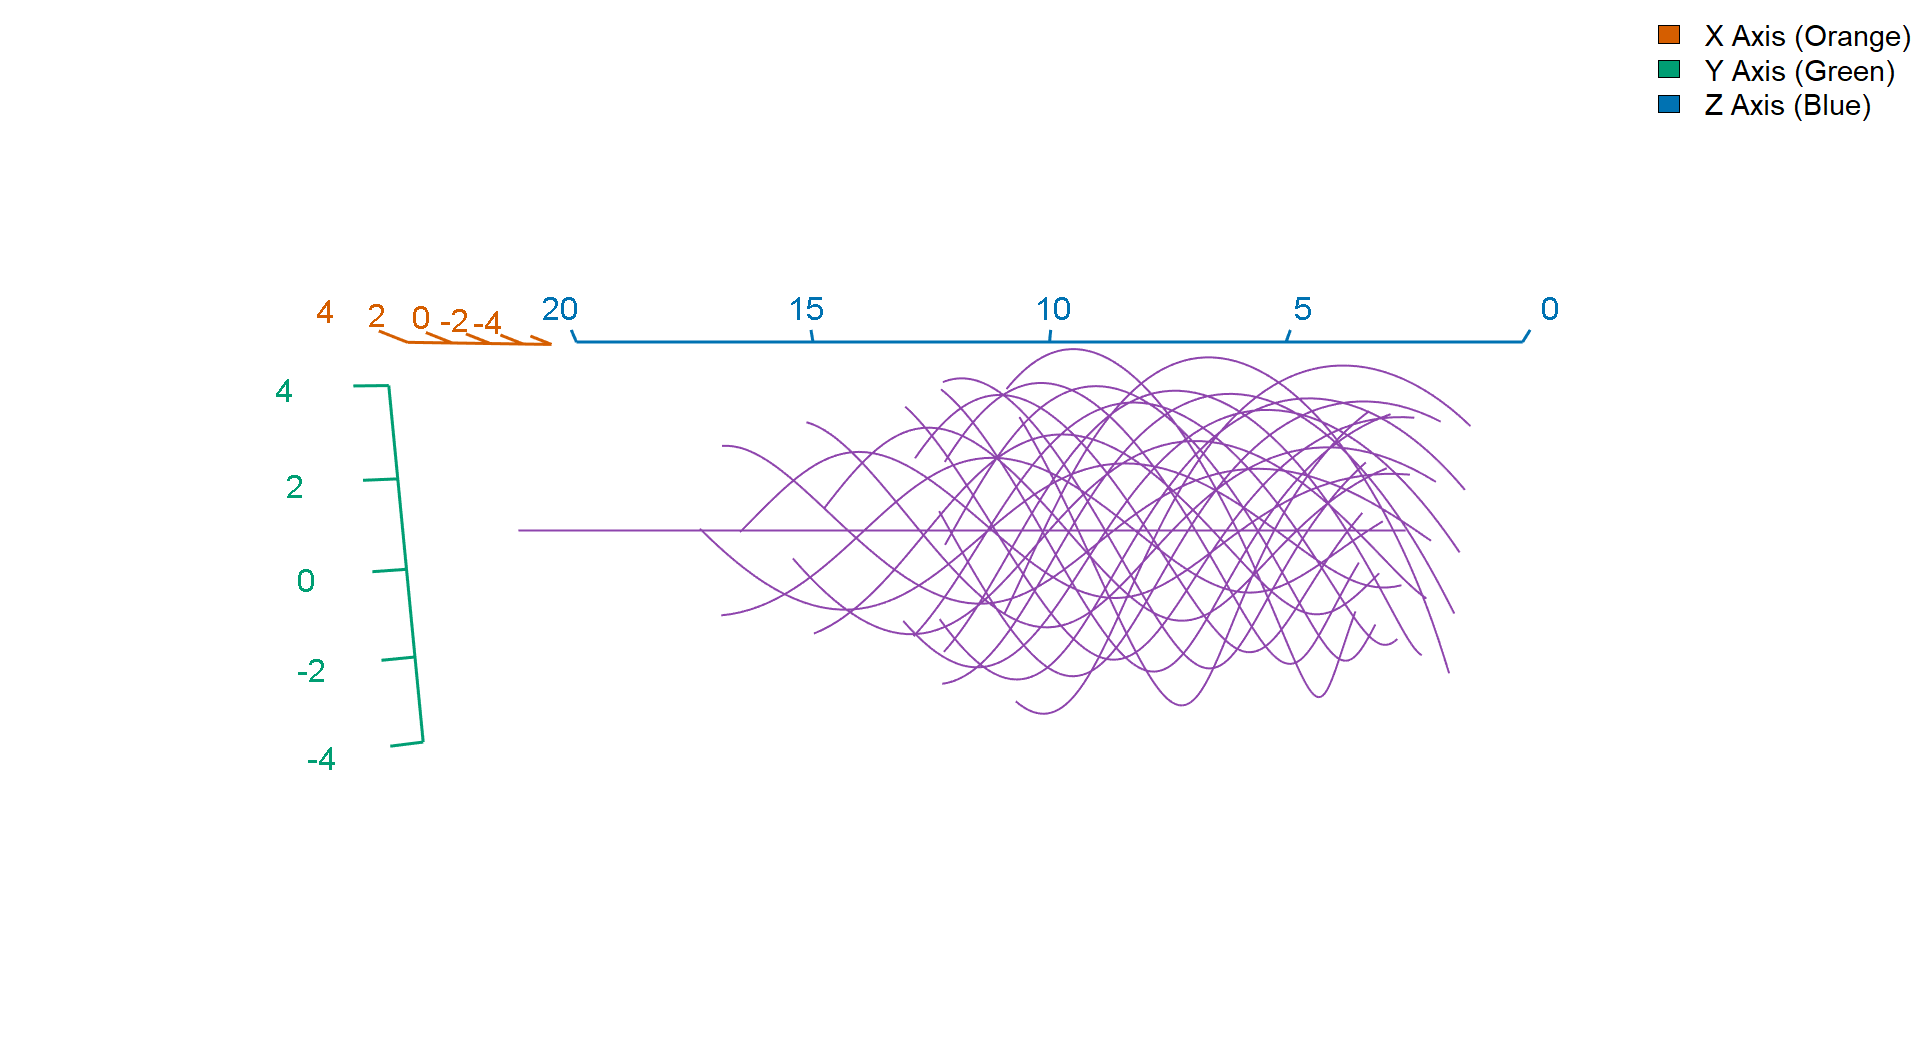
\includegraphics[width=0.85\textwidth]{vortex_view3.png}
		\caption{Lower-altitude view (View 3) emphasizing how horizontal wind direction evolves into vertical motion.}
		\label{fig:wind_streamlines_3}
	\end{figure}
	
	
	\vspace{1em}
\noindent
\textbf{Why this techniques matters:} \\
Vector field visualization helps explain system motion, direction, and interaction, such as airflow over a wing, magnetic field propagation, and turbulent ocean currents. These methods illuminate invisible forces for simulation, optimization, and design.

\vspace{0.5em}
\noindent
\textbf{It is used in:}
\begin{itemize}
    \item Airflow and turbulence simulations
    \item A study of electromagnetic fields
    \item Wind-current and oceanography modeling
    \item Analysis of mechanical and biomechanical motion
    \item Heat-transfer and combustion investigations
\end{itemize}

	\subsection{Combined Techniques}
	To gain deeper insights, scalar and vector visualization techniques can be combined. For example, streamlines can be rendered over scalar slice planes to show how flow interacts with scalar gradients. Isosurfaces can be layered with streaktubes to reveal vector behavior near scalar thresholds.
	
	Coloring streamlines by scalar values—such as using temperature to shade velocity paths—adds another layer of information. Combining multiple techniques must be done carefully to avoid clutter, but when done well, it enhances understanding significantly.

	This cohesive methodology is particularly advantageous in medical imaging (e.g., superimposing blood flow onto CT scans) or meteorology (e.g., integrating temperature gradients with wind vectors). Effectively constructed integrated visualizations can significantly enhance interpretability in time-critical domains such as disaster forecasting as shown in Figure~\ref{fig:earthquake_3d}.
	
		\begin{figure}[H]
		\centering
		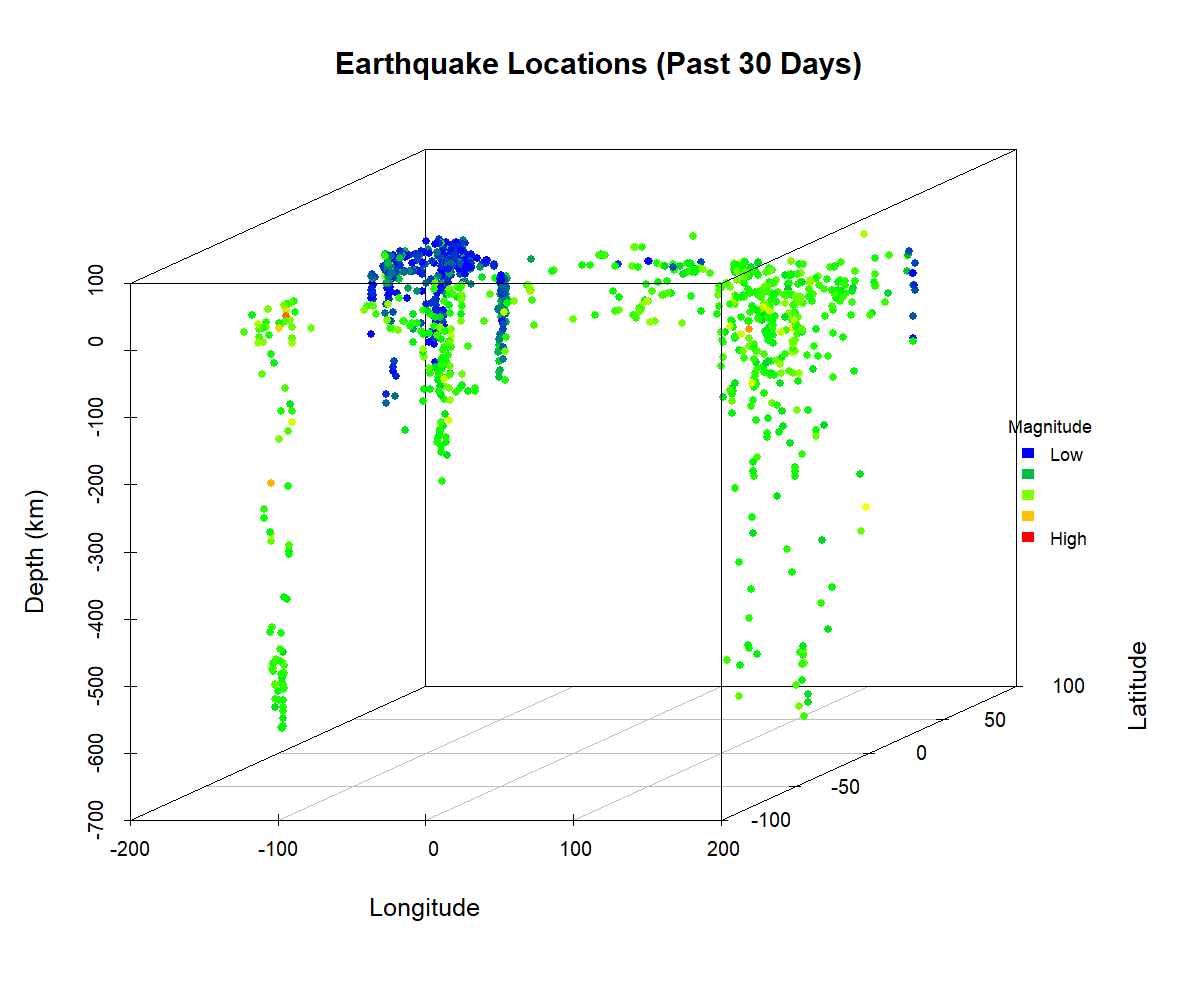
\includegraphics[width=0.95\textwidth]{earthquake_3d_plot_with_legend.png}
		\caption{3D scatter plot of global earthquake locations from the past 30 days. Depth is inverted for clarity. Color represents magnitude from low (blue) to high (red).}
		\label{fig:earthquake_3d}
	\end{figure}
	
	\vspace{1em}
	\noindent
	\textbf{Scenario: Real-World Seismic Event Data} \\
	This graph presents a real-world scientific visualization of spatial earthquake data, obtained from the USGS earthquake feed. Each point represents an earthquake, plotted by its longitude, latitude, and depth. The depth axis is inverted to reflect how earthquakes occur beneath Earth's surface. Color encodes scalar values (magnitude), transitioning from blue (low magnitude) to red (high magnitude).
	
	\vspace{0.5em}
	\noindent
	\textbf{Relation to Scientific Visualization} \\
	This plot illustrates a combined visualization approach, integrating both scalar and spatial vector information in one 3D scatter plot. It highlights how scalar data (magnitude) can be layered into positional 3D spatial domains. This kind of visualization is essential in geoscience and hazard monitoring, where both position and intensity influence understanding.
	
	\vspace{0.5em}
	\noindent
	\textbf{Why combining this techniques matters} \\
	By visually encoding magnitude through color and preserving geographic position and depth in 3D space, this approach allows researchers to analyze trends in earthquake clustering, depth zones, and magnitude distribution. Compared to traditional 2D maps, this 3D representation better reflects the spatial dynamics of seismic activity, supporting both qualitative insight and quantitative analysis.
	
	
	\subsection{Comparison Tables}
	
		\begin{table}[H]
		\centering
		\caption{Visualization Techniques: Data Type and Strength}
		\renewcommand{\arraystretch}{1.3}
		\begin{tabular}{|l|l|l|}
			\hline
			\textbf{Technique} & \textbf{Type} & \textbf{Strength} \\

			Slice Plane        & Scalar        & Simple, direct view \\

			Isosurface         & Scalar        & Highlights scalar thresholds \\

			Volume Rendering   & Scalar        & Full 3D view with transparency \\

			Scalar Glyphs      & Scalar        & Shows local values precisely \\

			Vector Glyphs      & Vector        & Explicit direction + magnitude \\

			Streamlines        & Vector        & Smooth, clean flow depiction \\

			Streaktubes        & Vector        & Adds 3D thickness and depth \\

			Ribbons            & Vector        & Shows twist and vorticity \\
			\hline
		\end{tabular}
	\end{table}
	
	\noindent Table 1 summarizes the classification and general strength of each visualization technique.
	
	\vspace{3em}
	
	\begin{table}[H]
		\centering
		\caption{Visualization Techniques: Advantages and Limitations}
		\renewcommand{\arraystretch}{1.3}
		\begin{tabular}{|l|l|l|}
			\hline
			\textbf{Technique} & \textbf{Advantage} & \textbf{Limitation} \\

			Slice Plane        & Great for detecting cross-sectional variation & Only 2D \\

			Isosurface         & Captures 3D boundary regions effectively      & Hard to read when nested \\

			Volume Rendering   & Reveals internal structures holistically     & Needs careful opacity control \\

			Scalar Glyphs      & Useful in sparse or boundary data            & Cluttered in dense regions \\

			Vector Glyphs      & Direct and intuitive for small datasets      & Visually cluttered in high density \\

			Streamlines        & Good for path tracking in steady fields      & Doesn't show magnitude directly \\

			Streaktubes        & Easier to follow in 3D space                 & More complex rendering \\

			Ribbons            & Ideal for rotational fields and turbulence   & Direction can be ambiguous \\
			\hline
		\end{tabular}
	\end{table}
	
	\noindent Table 2 evaluates the practical advantages and limitations of each method in real-world use.
	
	\section{Conclusion}
	Scientific visualization techniques are essential tools for interpreting multidimensional data. Slice planes and isosurfaces are effective for scalar fields, while streamlines and ribbons reveal patterns in vector fields. Combining methods, especially when enhanced with color and transparency, offers rich insights that surpass the capabilities of any single technique. This survey highlights the value of choosing appropriate visual tools based on data type, density, and research goals.
	
	\section{References}
	
	\begin{thebibliography}{9}
		\bibitem{hansen} Hansen, C. D., \& Johnson, C. R. (2005). \textit{The Visualization Handbook}. Elsevier.
		\bibitem{schroeder} Schroeder, W., Martin, K., \& Lorensen, B. (2006). \textit{The Visualization Toolkit}. Kitware.
		\bibitem{ware} Ware, C. (2020). \textit{Information Visualization: Perception for Design}. Morgan Kaufmann.
		\bibitem{matplotlib} Hunter, J. D. (2007). Matplotlib: A 2D graphics environment. \textit{Computing in Science \& Engineering}, 9(3), 90-95.
		\bibitem{rvis} Wickham, H. (2016). \textit{ggplot2: Elegant Graphics for Data Analysis}. Springer.
		\bibitem{usgsdata}
		U.S. Geological Survey (USGS). Earthquake Catalog Data Feed. \url{https://earthquake.usgs.gov/earthquakes/feed/v1.0/summary/all_month.csv}. Accessed April 13, 2025.
		\bibitem{openmeteo} Open-Meteo API. \url{https://open-meteo.com/}
		
	\end{thebibliography}
	
\end{document}
